\documentclass[10pt,twocolumn]{article}

\usepackage{times}
\usepackage{spverbatim}
\usepackage[swedish]{babel}
\usepackage[utf8]{inputenc}
\usepackage{listings}
\usepackage[toc,page]{appendix}
\usepackage{graphicx}
\usepackage{mathtools}
\usepackage{float}
\usepackage[margin={2.45cm, 2.45cm}]{geometry}
\renewcommand\appendixname{Bilagor}
\renewcommand\appendixpagename{Bilagor}
\usepackage[compact]{titlesec}
\titlespacing{\section}{0pt}{*2}{*2}
\raggedbottom
\sloppy

\title{Laborationsrapport i TSKS10 \emph{Signaler, Information och Kommunikation}}

\author{Martin Söderén \\ marso329, 9009291098 }

\date{\today}

\begin{document}

\maketitle

\clearpage

\section{Inledning}

Den här laborationen gick ut på analysera en delvis okänd signal. En del saker om den var givna men en del som krävdes för att kunna lyssna på signalen behövdes bestämmas experimentellt. Signalen ser ut på följande sätt:
$$x(t)=x_I(t)\cos(2\pi f_c t)-x_Q(t)\sin(2\pi f_c t)+z(t)$$
Där de intressanta signalerna är $X_I(t)$ och $X_Q(t)$. Båda dessa signaler innehåller en melodi, ett ordspråk och slutligen vitt brus. $z(t)$ betecknar signaler som sändaren skickar ut på andra bärfrekvenser.

\begin{itemize}
\item Bärfrekvensen $f_c$ är en multipel av 19 kHz
\item Signalen studsar mot ett objekt så att ett eko uppstår. Tiden $\tau_1$ är tiden det tar från sändaren till mottagaren direkt. Tiden $\tau_2$ är tiden det tar från sändare till objekt och sedan till mottagare. $\tau_2>\tau_1$ samt $\tau_2-\tau_1$ är en multipel av 1 ms. 
\item Ekot gör att vi tar emot $y(t)=x(t-\tau_1)+0,9x(t-\tau_2)$
\item Signalen tas emot lågpassfiltrerad med ett idealt lågpassfilter. Samplingsfrekvensen är 400 kHz.
\end{itemize}

Målet med laborationen är att demodulera signalen samt hantera ekot och därefter identifiera ordspråken.

\section{Metod}

Uppgiften delades upp i tre mindre uppgifter:

\begin{enumerate}
\item Ta reda på bärfrekvensen $f_c$
\item Ta reda på tidsfördröjningen $\tau_2-\tau_1$ samt eliminera ekot
\item I/Q-demodulera signalen
\end{enumerate}

MATLAB användes som verktyg för att lösa uppgiften. Koden återfinns i bilaga \ref{app:code}.

\subsection{Bärfrekvens} \label{sec:carrier}
För att få fram bärfrekvensen så fouriertransformerades signalen och dess amplitudspektrum studerades. Detta kan ses i figur \ref{fig:amplitud}.
Här ser man tre tydliga toppar. Dessa är vid 57000, 95000 och 133000 Hz, vilka alla är multipler av 19 kHz.

Signalen filtreras genom tre bandpassfilter för att få ut respektive smalbandssignal. De tre smalbandssignalerna kan ses i figur \ref{fig:tid}.

Den första signalen (57 kHz) ser ut att bara innehålla vitt brus. Den tredje (133 kHz) verkar också innehålla något brusliknande. Den andra signalen (95 kHz) verkar vara den sökta, den är uppdelad i tre distinkta delar som skulle kunna motsvara en melodi, tal och brus. Därmed används bärfrekvensen $f_c = 95$ kHz.

\subsection{Tidsfördröjning}
För att få fram ekots tidsfördröjning i signalen så autokorreleras det vita bruset från den första signalen med bärfrekvens 57 kHz. I figur \ref{fig:eko} så kan man se en topp vid 0 s och två sidotoppar $\pm 0.42 $ s på varje sida om huvudtoppen. Detta ger att $\Delta \tau=|\tau_{2}-\tau_{1}|=0.42$. Denna metod beskrivs och förklaras i kursboken kapitel 4.

\subsection{Filtrera bort eko}
Då $\Delta \tau$ och ekots amplitud nu är kända kan ekot filtreras bort. Detta görs genom att $x_1(t)=y(t)-0.9y(t-\Delta \tau) \text{ för alla } t>\Delta \tau$. I implementationen sker detta dock i block istället för varje enskilt sampel för att skynda på exekveringen. Efter filtreringen är signalen $x_1(t)$  kvar. När ekot filtreras bort så bortser vi från $\tau_1$ då vi vet att $\tau_1$ kommer ge en fasförskjutning på $X_I(t)$ och $X_Q(t)$ med $-2\pi f_c\tau_1$.

\subsection{I/Q-demodulering}
Signalen I/Q-demoduleras på följande sätt från kursboken avsnitt 1.4.2 med den extra fasförskjutningen:
$$ x_I(t)= \mathcal{H}^{LP}_{B/2}\{ 2x_1(t)\cos(2 \pi f_c t -2\pi f_c\tau_1) \}$$
$$ x_Q(t)= -\mathcal{H}^{LP}_{B/2}\{ 2x_1(t)\sin(2 \pi f_c t -2\pi f_c\tau_1) \}$$
Där $B$ är signalens bandbredd som kan antas vara 20 kHz då signalen ska innehålla hörbart ljud. Bärfrekvensen $f_c$ är känd från avsnitt \ref{sec:carrier} och är 95 kHz. Detta gav oss basbandssignalerna $x_I(t)$ och $x_Q(t)$ som fortfarande har en fasförskjutning. Vi vet att fasförskjutningen begränsas av 0 och $\pi/2$ då en större fasförskjutning än $\pi/2$ gör att $x_I(t)$ och $x_Q(t)$ byter plats. Skulle en fasförskjutning existera skulle detta ledda till att ljudet från de olika signalerna hamnar ovanpå varandra vilket skulle göra det svårt att höra ljudet klart. I detta fall så hördes ljudet klart utan att ta hänsyn till fasförskjutningen. Hade detta inte varit fallet så hade fasförskjutningen testas fram tills dess att de två signalerna hördes klart och tydligt. Anledningen till att $\tau_1$ har införts är för att det är tiden det tar för signalen att nå mottagaren och detta kan estimeras med en fasförskjutning, detta beskrivs i kursboken kapitel 1.4.2.  

\section{Resultat}

Den sökta informationen är:
\begin{itemize}
\item Bärfrekvensen $f_c$ är 95 kHz
\item Tidsfördröjningen $\tau_2-\tau_1$ är 420 ms.
\item I-signalen innehöll ordspråket "inget ont som inte har något gott med sig".
\item Q-signalen innehöll ordspråket "man ska inte kasta sten i glashus".
\end{itemize}


\begin{figure}[H]
	\begin{center}
		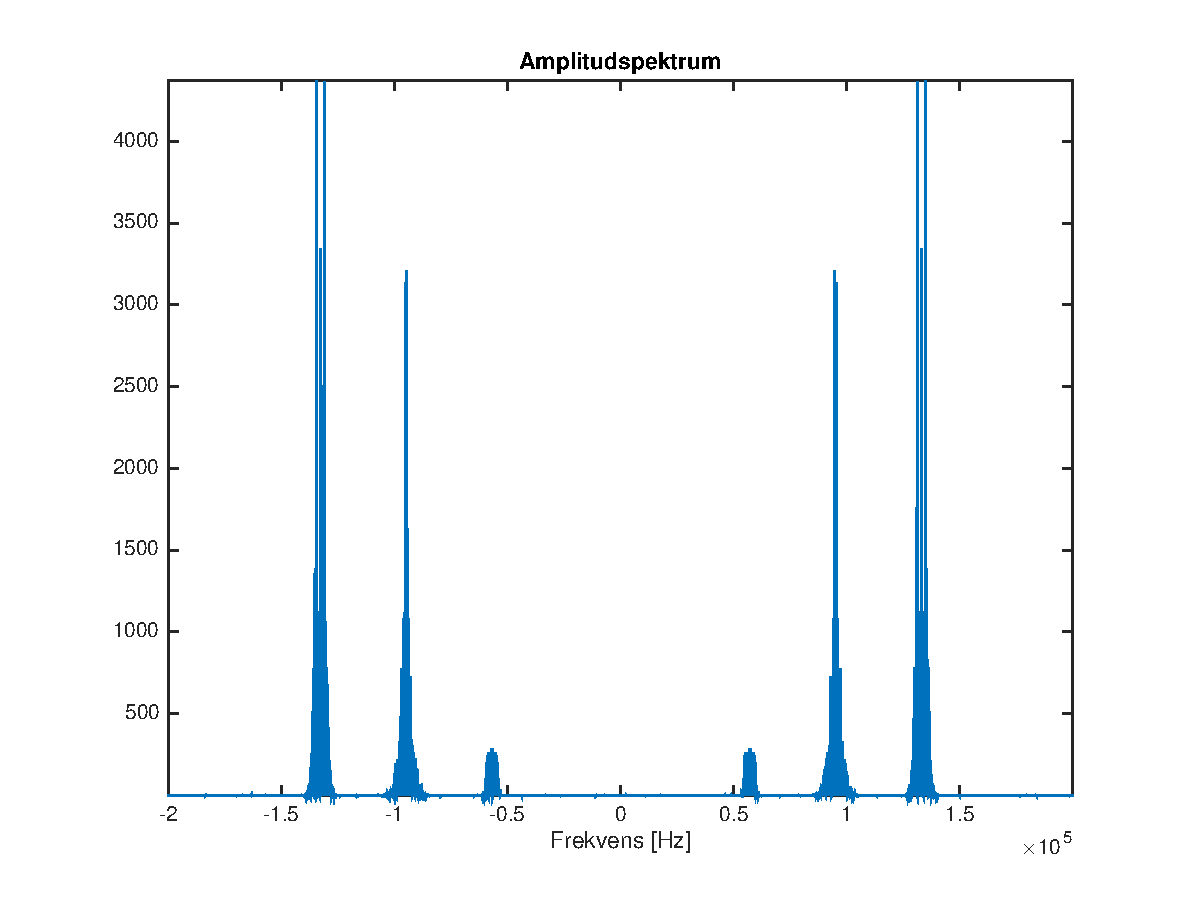
\includegraphics[scale=0.5]{figurer/amplitud.eps}
	\end{center}
	\caption{Fouriertranform av signalen.}
	\label{fig:amplitud}
\end{figure}

\begin{figure}[H]
	\begin{center}
		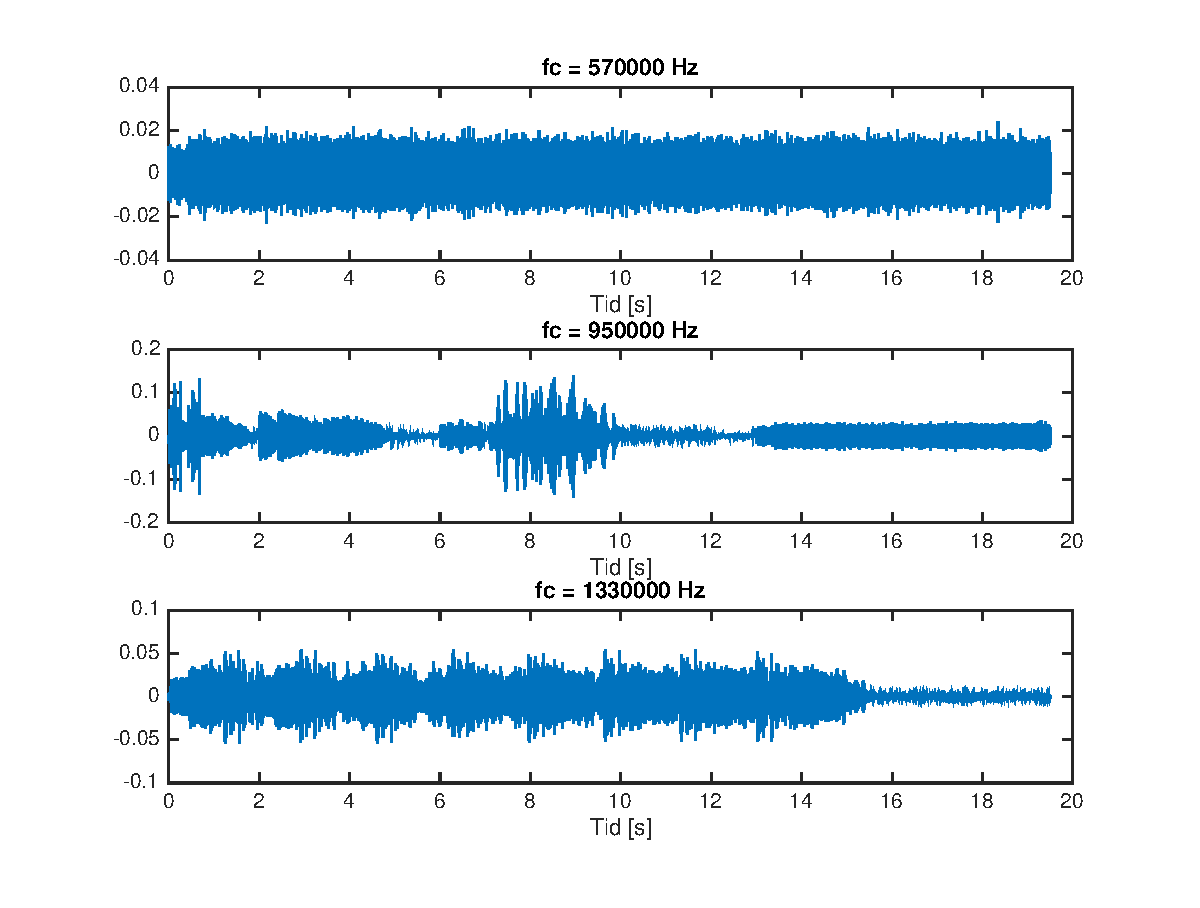
\includegraphics[scale=0.5]{figurer/tid.eps}
	\end{center}
	\caption{Smalbandssignalerna i tiddomänen.}
	\label{fig:tid}
\end{figure}

\begin{figure}[H]
	\begin{center}
		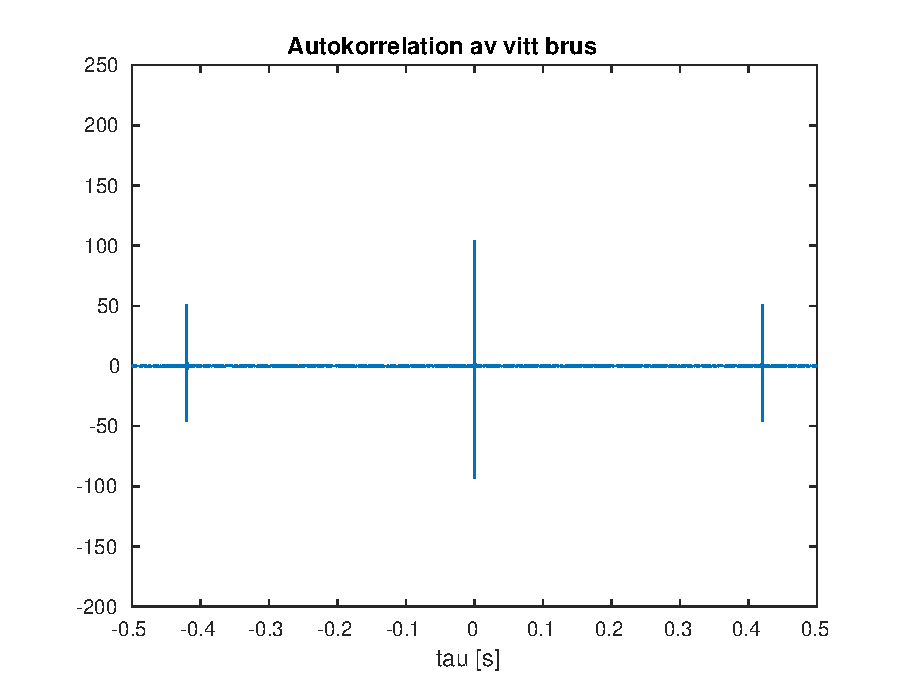
\includegraphics[scale=0.66]{figurer/eko.eps}
	\end{center}
	\caption{Autokorrelation av vitt brus.}
	\label{fig:eko}
\end{figure}

\newpage

\onecolumn
\appendix
\section{Min Matlab-kod} \label{app:code}
\lstinputlisting[language=matlab]{matlab/tsks10.m}
\end{document}
